\documentclass[a4paper,twoside,10pt]{scrreprt}

\usepackage{polyglossia}
\usepackage{pdfpages}
\usepackage{csquotes}
\usepackage{listings}
\lstset{language=C++,
                basicstyle=\ttfamily,
                keywordstyle=\color{blue}\ttfamily,
                stringstyle=\color{red}\ttfamily,
                commentstyle=\color{green}\ttfamily,
                morecomment=[l][\color{magenta}]{\#}}
\usepackage{abstract}
\usepackage{tikz}
\usetikzlibrary{matrix}
\usetikzlibrary{arrows}
\usepackage[headsepline]{scrlayer-scrpage}
\usepackage[backend=biber,style=alphabetic]{biblatex}
\addbibresource{sources.bib}
\setmainlanguage{german}
\usepackage{placeins}
%\usepackage{float}
\usepackage{amsmath}   
\usepackage{amsthm} 
\usepackage{mathtools}
\usepackage{amsfonts}
\usepackage{caption}
\usepackage{tabularx}
\usepackage{tabulary}
\usepackage{graphicx}
\usepackage{multirow}
\newcolumntype{Y}{>{\centering\arraybackslash}X}
\usepackage[german]{hyperref}
\usepackage[noabbrev,capitalize]{cleveref}
   
\pagestyle{scrheadings}
\ohead{\headmark}
\automark[chapter]{chapter}
\ofoot{\pagemark}

\DeclareMathOperator{\img}{im}
\newcommand{\UBC}{\text{UBC}}
\newcommand{\Z}{\mathbb{Z}}
\newcommand{\N}{\mathbb{N}}
\newcommand{\Q}{\mathbb{Q}}
\newcommand{\R}{\mathbb{R}}
\newcommand{\K}{\mathbb{K}}
\newcommand{\Inv}[1]{\text{Inv(}#1\text{)}}
%\newcommand{\Barf}{\text{Bar}}
\newcommand{\Hom}[2][]{\text{Hom}%
\ifthenelse{\equal{#1}{}}{}{_{#1}}%
\left(#2\right)}%
\newcommand{\pre}[2]{\prescript{}{#1}{\text{#2}]}}
\newcommand{\BHom}[2][]{\text{BHom}%
\ifthenelse{\equal{#1}{}}{}{_{#1}}%
\bigl(#2\bigr)}%

\renewcommand{\sectfont}{\normalfont}

\newtheorem{satz}{Satz}[section]
\newtheorem{lemma}[satz]{Lemma}
\newtheorem{korollar}[satz]{Korollar}
\theoremstyle{definition}
\newtheorem{definition}[satz]{Definition}
\newtheorem{bemerkung}[satz]{Bemerkung}
\newtheorem{aufgabe}[satz]{Aufgabe} 
\newenvironment{beweis}
    {\begin{proof}[Beweis]}
    {\end{proof}}
\newtheorem{beispiel}[satz]{Beispiel}
  
\newenvironment{proofsketch}
    {\begin{proof}[Sketch of proof]}
    {\end{proof}}

%  \author{Simon~Lang (\textsf{simon1.lang@uni-regensburg.de})}
%  \date{02.01.2020}
%  \title{Die Eigenschaft UBC auf freien Gruppen}
%%  \subtitle{Subtitle}

\begin{document}
\pagenumbering{gobble}
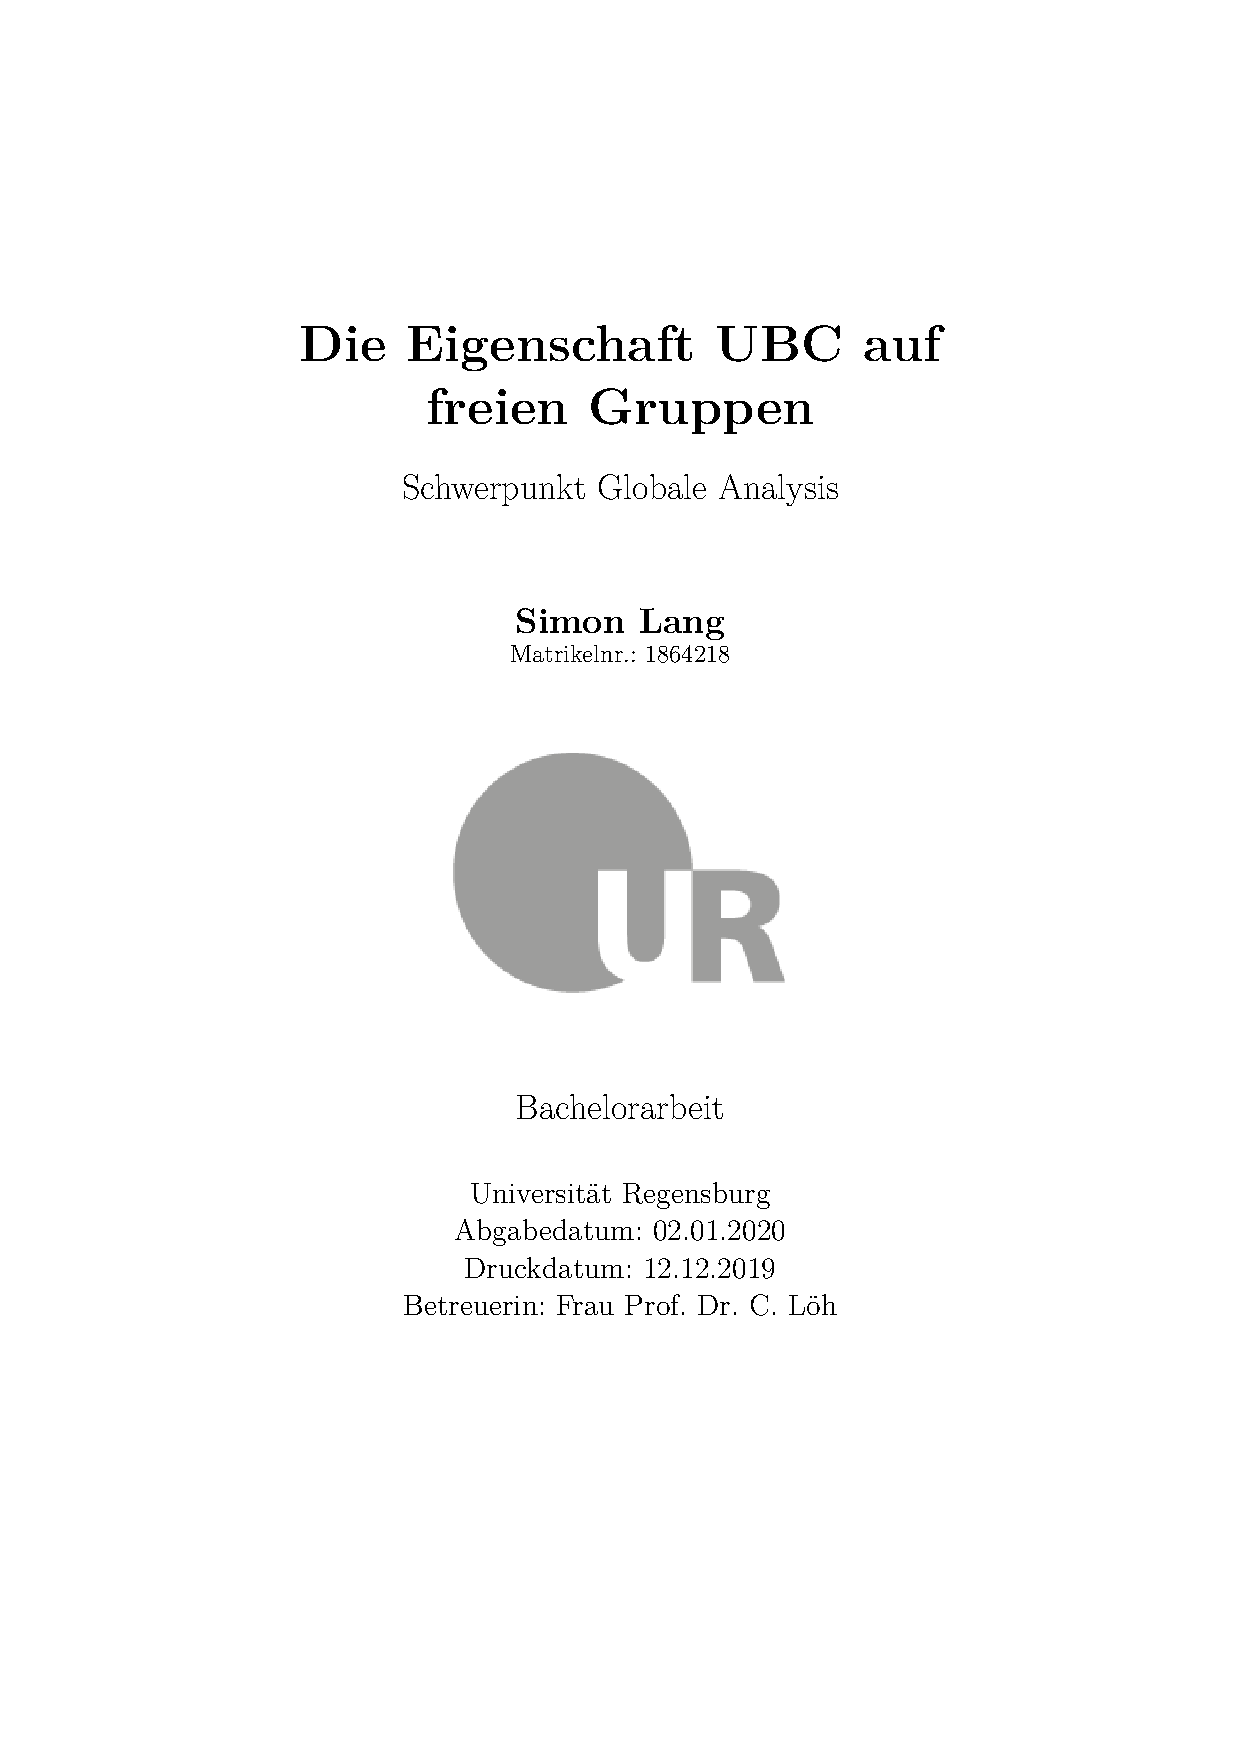
\includepdf{cover.pdf}
\begin{abstract}
Die Gruppenkohomologie für eine freie Gruppe $F_n$ von Rang $n$ ist vollständig bekannt. So gilt beispielweise mit $\R$-Koeffizienten (und trivialer Gruppenwirkung auf $\R$)
\begin{equation*}
H^q(F_n,\R)\cong
\begin{cases} 
      \R & q=0 \\
      \R^n & q=1 \\
      0 & q\geq 2
\end{cases}
\end{equation*}
Für den funktionalanalytischen Zwilling der Gruppenkohomologie, der beschränkten Kohomologie von Gruppen $H_b^*(G,\R)$, gilt dies jedoch nicht. Obwohl sich diese in niedrigen Graden sehr einfach bestimmen lässt und sogar unabhängig von der Gruppe $G$ ist (siehe \cref{sec:BoundedCohomInLowDeg}), ist sie bereits für $F_2$ für $q\geq 4$ unbekannt. \par
Für $q=2$ wurde von \autocite{mitsumatsu} und für $q=3$ wurde von \autocite{soma} gezeigt, dass $\dim_{\R} H_b^q(G,\R)=\infty$ gilt. Insbesondere demonstriert dies, dass beschränkte Kohomologie von Gruppen i.A. nichttrivial ist. Dies ist nicht offensichtlich, da sie nach \cite{gromov} für mittelbare Gruppen für $q>0$ verschwindet.\par
In dieser Arbeit werden zuerst die grundlegenden Begriffe für das  Setting von (Ko)Homologie definiert. Gruppenkohomologie und beschränkte Kohomologie von Gruppen werden anschließend über die Bar-Auflösung konstruiert.\par
Basierend auf \cite[Theorem 2.8]{matsumoto} wird mithilfe der ,,Uniform Boundary Condition'' (UBC) eine äquivalente Charakterisierung der Trivialität von $H_b^4(F_2,\R)$ bewiesen, welche einen experimentellen Zugang ermöglicht.\par
Zuletzt wird eine beispielhafte Implementation des Experiments in der Programmiersprache C++ gegeben und ein generierter Datensatz ausgewertet.
\end{abstract}
\tableofcontents
\newpage
\pagenumbering{arabic}
\chapter{Konstruktion der beschränkten Kohomologie von Gruppen}
Wir verwenden die folgenden Konventionen: Alle Ringe sind unitär, Moduln sind Links-Moduln (sofern nicht anders angegeben).\par
Wichtig sowohl für die Konstruktion der Gruppenkohomologie als auch der beschränkten Kohomologie von Gruppen ist der Gruppenring. Dazu definieren wir dessen universelle Eigenschaft und geben die konkrete Konstruktion im Spezialfall des Ringes $\Z$ an, da diese für unsere Zwecke genügt.

\section{Gruppenringe}
\begin{definition}[universelle Eigenschaft des Gruppenrings]\label{def:GroupRingUnivProperty}
Sei $R$ ein Ring. Der \emph{Gruppenring} $R[G]$ (der sogar die Struktur einer $R$-Algebra besitzt) besitzt zusammen mit der kanonischen Inklusion $i:G\to R[G]$ folgende universelle Eigenschaft:\par
Für jede $R$-Algebra $S$ und jeden Gruppenhomomorphismus $f:G\to S^{\times}$ existiert ein eindeutiger $R$-Algebrenhomomorphismus $R[f]:R[G]\to S$ mit $R[f]\circ i=(S^{\times} \xhookrightarrow{\text{incl}} S)\circ f$.
\begin{center}
\begin{tikzpicture}
  \matrix (m) [matrix of math nodes,row sep=3em,column sep=4em,minimum width=2em]
  {
     G & S^{\times} & S \\
     R[G] \\};
  \path[-stealth]
  
    (m-1-1) edge node [left] {$i$} (m-2-1)
            edge node [above] {$f$} (m-1-2)
    (m-2-1) edge [dashed] node [below right] {$\exists!~R[f]$} (m-1-3);
    \draw[right hook->] (m-1-2) -- node [above] {incl} (m-1-3);
\end{tikzpicture}
\end{center}
Diese universelle Eigenschaft entspricht der Tatsache, dass der Funktor $R[-]:\text{Grp}\to R\text{-Alg}$ linksadjungiert ist zu dem Funktor $(-)^{\times}:R\text{-Alg}\to \text{Grp}$, der eine $R$-Algebra auf ihre Einheitengruppe schickt.\par
Da wir uns meist nur für die Ringstruktur interessieren, sprechen wir vom Gruppenring.
\end{definition}

\begin{definition}[ganzzahliger Gruppenring]
Wir konstruieren im folgenden den Gruppenring $\Z[G]$. Für allgemeine Ringe verläuft die Konstruktion analog.\par
Sei $G$ eine Gruppe. Der (integrale) Gruppenring $\Z[G]$ von $G$ ist definiert wie folgt:\par
Die zugrundeliegende additive Gruppe ist die freie abelsche Gruppe $\bigoplus\limits_G \Z$, wobei wir $G$ als die kanonische Basis auffassen. Somit können wir $x\in \Z[G]$ als $x=\sum\limits_{g\in G}a_g\cdot g$ mit eindeutigen Koeffizenten $a_g \in \Z$ auffassen, die für alle bis auf endlich viele $g\in G$ verschwinden. Die Addition ist also gegeben durch die Abbildung 
\begin{align*}
+:\Z[G]\times \Z[G] &\to \Z[G]\\
\biggl(\sum\limits_{g\in G}a_g\cdot g, \sum\limits_{g\in G}b_g\cdot g\biggr) &\mapsto\sum\limits_{g\in G}(a_g+b_g)\cdot g
\end{align*}
und die Multiplikation durch
\begin{align*}
\cdot :\Z[G]\times \Z[G] &\to \Z[G]\\
\biggl(\sum\limits_{g\in G}a_g\cdot g, \sum\limits_{h\in G}b_h\cdot h\biggr) &\mapsto\sum\limits_{g\in G}\biggl(\sum\limits_{h\in G}a_hb_{h^{-1}g}\biggr)\cdot g.
\end{align*}
Da $1\cdot e$ (mit $e\in G$ neutrales Element) ein neutrales Element bezüglich der Multiplikation ist, ist $\Z[G]$ ein unitärer (aber nicht notwendigerweise kommutativer) Ring. (Die restlichen Ringaxiome lassen sich an der angegebenen Konstruktion verifizieren.)
\end{definition}

\section{Elementare Begriffe der homologischen Algebra}
Es gibt verschiedene Möglichkeiten Gruppenkohomologie bzw. beschränkte Kohomologie von Gruppen zu konstruieren. Da wir sie über die sogenannte Bar-Auflösung einführen werden, wiederholen wir Grundbegriffe der homologischen Algebra. Die hier benutzten Indexkonventionen gelten auch im weiteren Verlauf.
\begin{definition}[Kategorie der Kettenkomplexe]\label{def:CatChainComplex}
Sei $R$ ein Ring. Ein \emph{(Links-)$R$-Kettenkomplex} $C_*$ ist ein Paar $\left(\left(C_n \right)_{n\in \Z},\left(\partial_n:C_n\to C_{n-1}\right)_{n\in \Z}\right)$, wobei für alle $n\in \Z$ gelte:
\begin{itemize}
\item $C_n$ ist ein $R$-Links-Modul
\item $\partial_n:C_n\to C_{n-1}$ ist eine $R$-lineare Abbildung
\item $\partial_n\circ \partial_{n+1}=0$
\end{itemize}
Die Abbildung $\partial_n$ wird als Randoperator bezeichnet.
Die Kategorie $\prescript{}{R}{\text{Ch}}$ ist die Kategorie der (Links-)$R$-Kettenkomplexe, wobei die Objekte die eben definierten Kettenkomplexe sind und Morphismen $C_*\to D_*$ zwischen Kettenkomplexen gegeben sind durch Familien $(f_n:C_n\to D_n)_{n\in \Z}$, für die
\begin{center}
\begin{tikzpicture}
  \matrix (m) [matrix of math nodes,row sep=3em,column sep=4em,minimum width=2em]
  {
     C_n & C_{n-1} \\
     D_n & D_{n-1} \\};
  \path[-stealth]
    (m-1-1) edge node [left] {$f_n$} (m-2-1)
            edge node [above] {$\partial_n^C$} (m-1-2)
    (m-2-1) edge node [below] {$\partial_n^D$} (m-2-2)
    (m-1-2) edge node [right] {$f_{n-1}$} (m-2-2);
\end{tikzpicture}
\end{center}
kommutiert. Die Verknüpfung von Morphismen ist durch die gradweise Abbildungsverknüpfung gegeben.\par
Weiter bezeichnen wir im folgenden Elemente aus $C_n$ als \textit{(n-)Ketten}, Elemente aus $\ker\partial_n$ als \textit{(n-)Zykel} und Elemente aus $\img\partial_{n+1}$ als \textit{(n-)Ränder}.
\end{definition}

\begin{definition}[Homologie von Kettenkomplex]
Wir definieren für alle $n\in \Z$ Funktoren $H_n:\prescript{}{R}{\text{Ch}}\to \prescript{}{R}{\text{Mod}}$ wie folgt:
\begin{itemize}
\item auf Objekten:
\begin{equation*}
H_n(C_*):=\frac{\ker\partial_n}{\img\partial_{n+1}}
\end{equation*}
\item auf Morphismen:\par
Seien $C_*,D_*\in \text{Ob}(\prescript{}{R}{\text{Ch}})$ und $f\in \text{Hom}_{\prescript{}{R}{\text{Ch}}}(C_*,D_*)$. Dann ist 
\begin{align*}
H_n(f):H_n(C_*)&\to H_n(D_*)\\
[x]\mapsto [f(x)]
\end{align*}
eine wohldefinierte, $R$-lineare Abbildung. (Dies folgt aus der universellen Eigenschaft von Quotienten, da $f$ eine Kettenabbildung ist.)
\end{itemize}
Aus dieser Konstruktion folgt sofort, dass $H_n$ ein Funktor ist.
\end{definition}

\begin{definition}[Kategorie der Kokettenkomplexe]\label{def:CatCoChainComplex}
Sei $R$ ein Ring. Ein \emph{Links-)$R$-Kokettenkomplex} $C^*$ ist ein Paar $\left(\left(C^n \right)_{n\in \Z},\bigl(\delta^n:C^n\to C^{n+1}\right)_{n\in \Z}\bigr)$, wobei für alle $n\in \Z$ gelte:
\begin{itemize}
\item $C^n$ ist ein $R$-Links-Modul
\item $\delta^n:C^n\to C^{n+1}$ ist eine $R$-lineare Abbildung
\item $\delta^n\circ \delta^{n-1}=0$
\end{itemize}
Die Abbildung $\delta^n$ wird als Korandoperator bezeichnet.
Die Kategorie $\prescript{}{R}{\text{KoCh}}$ ist die Kategorie der (Links-)$R$-Kokettenkomplexe, wobei die Objekte die eben definierten Kokettenkomplexe sind und Morphismen $C^*\to D^*$ zwischen Kokettenkomplexen gegeben sind durch Familien $(f_n:C^n\to D^n)_{n\in\Z}$, für die
\begin{center}
\begin{tikzpicture}
  \matrix (m) [matrix of math nodes,row sep=3em,column sep=4em,minimum width=2em]
  {
     C^n & C^{n+1} \\
     D^n & D^{n+1} \\};
  \path[-stealth]
    (m-1-1) edge node [left] {$f_n$} (m-2-1)
            edge node [above] {$\delta_C^n$} (m-1-2)
    (m-2-1) edge node [below] {$\delta_D^n$} (m-2-2)
    (m-1-2) edge node [right] {$f_{n+1}$} (m-2-2);
\end{tikzpicture}
\end{center}
kommutiert. Die Verknüpfung von Morphismen ist wieder durch die gradweise Abbildungsverknüpfung gegeben.\par
Weiter bezeichnen wir im folgenden Elemente aus $C^n$ als \textit{(n-)Koketten}, Elemente aus $\ker\delta^n$ als \textit{(n-)Kozykel} und Elemente aus $\img\delta^{n-1}$ als \textit{(n-)Koränder}.
\end{definition}

\begin{definition}[Kohomologie von Kokettenkomplex]\label{def:DefCohomCochain}
Wir definieren für alle $n\in \Z$ Funktoren $H^*:\prescript{}{R}{\text{KoCh}}\to \prescript{}{R}{\text{Mod}}$ wie folgt:
\begin{itemize}
\item auf Objekten:
\begin{equation*}
H^n(C^*):=\frac{\ker\delta^n}{\img\delta^{n-1}}
\end{equation*}
\item auf Morphismen:\par
Seien $C^*,D^*\in \text{Ob}(\prescript{}{R}{\text{KoCh}})$ und $f\in \text{Hom}_{\prescript{}{R}{\text{KoCh}}}(C^*,D^*)$. Dann ist 
\begin{align*}
H^n(f):H^n(C^*)&\to H^n(D^*)\\
[x]\mapsto [f(x)]
\end{align*}
eine wohldefinierte, lineare Abbildung. (Dies folgt aus der universellen Eigenschaft von Quotienten, da $f$ eine Kokettenabbildung ist.)
\end{itemize}
Aus dieser Konstruktion folgt sofort, dass $H^n$ ein Funktor ist.
\end{definition}
Im folgenden wird häufig der Fall von (Ko)Kettenkomplexen auftreten, die über $\N$ statt $\Z$ indiziert sind. In diesem Fall sind die verbleibenden Indizes mit Nullmoduln und trivialen (Ko)Randoperatoren zu ergänzen. Wir benutzen für Kettenkomplexe und Homologie untere Indices sowie obere Indices für Kokettenkomplexe und Kohomologie.

\section{Bar-Auflösung und elementare Eigenschaften}
Im folgenden sei $G$ eine Gruppe.
Wir definieren nun die Bar-Auflösung $C_*(G)$ der Gruppe $G$. Auf dieser Konstruktion aufbauend werden wir sowohl Gruppenkohomologie als auch beschränkte Kohomologie von Gruppen konstruieren.
\begin{definition}[Die Bar-Auflösung $C_*(G)$]\label{def:BarRes}
Für $n\in \N$ definiere
\begin{equation*}
C_n(G):=\bigoplus_{G^n} \Z[G]
\end{equation*}
d.h. $C_n(G)$ sei der freie $\Z[G]$ Modul zur Basis $G^n$. Wir notieren die Elemente der $\Z[G]$-Basis $(g_1,\ldots,g_n)$ als $[g_1|\ldots|g_n]$ und das (einzige) Element der (trivialen) Gruppe $G^0$ als $[]$.
Die Randoperatoren seien definiert als
\begin{align*}
\partial_n:C_n(G)&\to C_{n-1}(G)\\
[g_1|\ldots|g_n]&\mapsto g_1\cdot [g_2|\ldots|g_n]\\ 
&+\sum\limits_{i=1}^{n-1} (-1)^i\cdot [g_1|\ldots|g_{i-1}|g_i\cdot g_{i+1}|g_{i+2}|\ldots|g_n]\\
&+(-1)^n\cdot [g_1|\ldots|g_{n-1}].
\end{align*}
Dass dies wirklich Randoperatoren sind wird in \cref{lem:ProofBarIsChainComplex} bewiesen.
%\\\noindent
%Seien nun $G,H\in Ob(\text{Grp})$ Gruppen und $\phi:G\to H$ ein Gruppenhomorphismus. Dann ist die Familie (der $\Z$-linearen Fortsetzungen von)
%\begin{align*}
%	C_n(\phi):C_n(G)&\to C_n(H)\\
%	g\cdot[g_1|\ldots|g_n]&\mapsto \phi(g)\cdot[\phi(g_1)|\ldots|\phi(g_n)]
%\end{align*}
%ein $\Z$-Kettenmorphismus.
\end{definition}

\begin{lemma}\label{lem:ProofBarIsChainComplex}
Die Bar-Auflösung aus \cref{def:BarRes} ist ein Kettenkomplex, d.h. $\partial_n\circ \partial_{n+1}=0$.
\begin{proof}
Es genügt zu zeigen, dass $\partial_n\circ \partial_{n+1}$ auf der kanonischen Basis von $C_{n+1}(G)$ verschwindet.\par
Um die Rechnung übersichtlich zu halten, führen wir unter der Konvention $n<m\Longrightarrow\sum\limits_{i=m}^n (\ldots)=0$ folgende Zerlegungen ein:
\par Es gilt
\begin{align*}
\partial_n\circ \partial_{n+1}([g_1|\ldots|g_{n+1}])&=g_1\cdot\partial_n([g_2|\ldots|g_{n+1}])\\ 
&+\sum\limits_{i=1}^n (-1)^i\cdot\partial_n([g_1|\ldots|g_{i-1}|g_i\cdot g_{i+1}|g_{i+2}|\ldots|g_{n+1}])\\
&+(-1)^{n+1}\cdot\partial_n([g_1|\ldots|g_n])
\end{align*}
und wir zerlegen die Summe in folgende Teile:
\begin{align*}
A:=&g_1\cdot\partial_n([g_2|\ldots|g_{n+1}])\\
=&g_1\cdot g_2\cdot [g_3|\ldots|g_{n+1}]+\sum\limits_{i=1}^{n-1}(-1)^i g_1\cdot[g_2|\ldots|g_{i+1}\cdot g_{i+2}|\ldots|g_{n+1}]\\
+&(-1)^n g_1\cdot[g_2|\ldots|g_{n}]\\
B:=&\sum\limits_{i=1}^n (-1)^i\cdot\partial_n([g_1|\ldots|g_{i-1}|g_i\cdot g_{i+1}|g_{i+2}|\ldots|g_{n+1}])\\
C:=&(-1)^{n+1}\cdot\partial_n([g_1|\ldots|g_n]).
\end{align*}
Weiter zerlegen wir 
\begin{align*}
\sum\limits_{i=1}^n (-1)^i\cdot\partial_n([g_1|&\ldots|g_i\cdot g_{i+1}|\ldots|g_{n+1}])\overset{\text{umordnen}}{=}-g_1\cdot g_2\cdot [g_3|\ldots|g_{n+1}]\\
&+\sum\limits_{i=2}^{n}(-1)^i g_1\cdot [g_2|\ldots|g_i\cdot g_{i+1}|\ldots|g_{n+1}]\\
&+\sum\limits_{i=3}^n\sum\limits_{j=1}^{i-2}(-1)^{i+j}\cdot [g_1|\ldots |g_j\cdot g_{j+1}|\ldots |g_i\cdot g_{i+1}|\ldots |g_{n+1}]\\
&+\sum\limits_{i=1}^{n-2}\sum\limits_{j=i+1}^{n-1}(-1)^{i+j}\cdot [g_1|\ldots|g_i\cdot g_{i+1}|\ldots|g_{j+1}\cdot g_{j+2}|\ldots|g_{n+1}]\\
&-\sum\limits_{i=2}^n [g_1|\ldots|g_{i-1}\cdot g_{i}\cdot g_{i+1}|\ldots|g_{n+1}]\\
&+\sum\limits_{i=1}^{n-1}[g_1|\ldots|g_i\cdot g_{i+1}\cdot g_{i+2}|\ldots|g_{n+1}]\\
&+\sum\limits_{i=1}^{n-1}(-1)^{i+n}\cdot [g_1|\ldots|g_i\cdot g_{i+1}|\ldots|g_n]+[g_1|\ldots|g_{n-1}]
\end{align*}
in 
\begin{align*}
B_1&:=-g_1\cdot g_2\cdot [g_3|\ldots|g_{n+1}]+\sum\limits_{i=2}^{n}(-1)^i g_1\cdot [g_2|\ldots|g_i\cdot g_{i+1}|\ldots|g_{n+1}]\\
B_2&:=\sum\limits_{i=3}^n\sum\limits_{j=1}^{i-2}(-1)^{i+j}\cdot [g_1|\ldots |g_j\cdot g_{j+1}|\ldots |g_i\cdot g_{i+1}|\ldots |g_{n+1}]\\
B_3&:=\sum\limits_{i=1}^{n-2}\sum\limits_{j=i+1}^{n-1}(-1)^{i+j}\cdot [g_1|\ldots|g_i\cdot g_{i+1}|\ldots|g_{j+1}\cdot g_{j+2}|\ldots|g_{n+1}]\\
B_4&:=-\sum\limits_{i=2}^n [g_1|\ldots|g_{i-1}\cdot g_{i}\cdot g_{i+1}|\ldots|g_{n+1}]\\
B_5&:=\sum\limits_{i=1}^{n-1}[g_1|\ldots|g_i\cdot g_{i+1}\cdot g_{i+2}|\ldots|g_{n+1}]\\
B_6&:=\sum\limits_{i=1}^{n-1}(-1)^{i+n}\cdot [g_1|\ldots|g_i\cdot g_{i+1}|\ldots|g_n]+[g_1|\ldots|g_{n-1}]\\
\end{align*}
und 
\begin{align*}
(-1)^{n+1}\cdot\partial_n([g_1|\ldots|g_n])&=(-1)^{n+1}g_1\cdot[g_2|\ldots|g_n])\\
&+\sum\limits_{i=1}^{n-1}(-1)^{i+n+1}\cdot [g_1|\ldots|g_i\cdot g_{i+1}|\ldots|g_n]\\
&-[g_1|\ldots|g_{n-1}]
\end{align*}
in
\begin{align*}
C_1&:=(-1)^{n+1}g_1\cdot[g_2|\ldots|g_n])\\
C_2&:=\sum\limits_{i=1}^{n-1}(-1)^{i+n+1}\cdot [g_1|\ldots|g_i\cdot g_{i+1}|\ldots|g_n]-[g_1|\ldots|g_{n-1}].
\end{align*}
Offenbar gilt $B_4+B_5=0$, $B_6+C_2=0$ und $A+B_1+C_1=0$.\par
Es gilt $B_3=-B_2$, denn
\begin{align*}
B_3&=\sum\limits_{i=1}^{n-2}\sum\limits_{j=i+1}^{n-1}(-1)^{i+j}\cdot [g_1|\ldots|g_i\cdot g_{i+1}|\ldots|g_{j+1}\cdot g_{j+2}|\ldots|g_{n+1}]\\
&\overset{\text{umordnen}}{=}\sum\limits_{j=2}^{n-1}\sum\limits_{i=1}^{j-1}(-1)^{i+j}\cdot [g_1|\ldots|g_i\cdot g_{i+1}|\ldots|g_{j+1}\cdot g_{j+2}|\ldots|g_{n+1}]\\
&=\sum\limits_{j=3}^n\sum\limits_{i=1}^{j-2}(-1)^{i+j-1}\cdot [g_1|\ldots|g_i\cdot g_{i+1}|\ldots|g_j\cdot g_{j+1}|\ldots|g_{n+1}]=-B_2 ,
\end{align*}
womit $\partial_n\circ \partial_{n+1}([g_1|\ldots|g_{n+1}])=0$ folgt.
\end{proof}
\end{lemma}

\begin{satz}[Eine $\Z$-Basis der Bar-Auflösung]\label{satz:ZBasisOfBarRes}
Die $\Z [G]$-Moduln $C_n(G)$ der Bar-Auflösung besitzen eine $\Z$-Basis und diese ist für $n\in \N$ gegeben durch $\{g_0\cdot [g_1|\ldots|g_n]\in C_n(G):(g_0,g_1,\ldots,g_n)\in G^{n+1}\}\subset C_n(G)$.
\begin{proof}
Nach Konstruktion gilt $C_n(G)=\bigoplus\limits_{G^n} \Z[G]$ und $\Z[G]\cong_{\prescript{}{\Z}{\text{Mod}}}\bigoplus\limits_{g\in G} \Z$. Wenn wir also $\Z[G]$ als $\Z$-Modul auffassen, gilt 
\begin{equation*}
C_n(G)=\bigoplus\limits_{G^n} \Z[G]\cong_{\prescript{}{\Z}{\text{Mod}}}\bigoplus\limits_{G^n}\bigoplus\limits_G \Z\cong_{\prescript{}{\Z}{\text{Mod}}}\bigoplus\limits_{G^{n+1}} \Z
\end{equation*}
wobei wir die angegebene Basis erhalten, indem wir die kanonische Basis von $\bigoplus\limits_{G^{n+1}} \Z$ ,,rückwärts'' durch die Isomorphismen auf $C_n(G)$ zurückführen.
\end{proof}
\end{satz}

\section{Wechseln der Koeffizienten}
Wir wollen im folgenden die Koeffizienten der Bar-Auflösung in $\R[G]$ bzw. $\Q[G]$ ändern. 
\begin{definition}[Tensorprodukt Modul und Kettenkomplex]\label{def:TensorModCh}
Seien $R,S$ Ringe und $M\in \prescript{}{S}{\text{Mod}}_R$, d.h. ein $(S,R)$-Bimodul. Weiter sei $C\in \prescript{}{R}{\text{Ch}}$.
Das Tensorprodukt $M\otimes_{R}C$ sei definiert als die Anwendung von $M\otimes_{R}(-)$ auf die Moduln und Randoperatoren des Kettenkomplexes. Aus der Funktorialität von $M\otimes_{R}(-):\prescript{}{R}{\text{Mod}}\to \prescript{}{S}{\text{Mod}}$ folgt bereits die Funktorialität $\prescript{}{R}{\text{Ch}}\to \prescript{}{S}{\text{Ch}}$, da das Tensorprodukt Nullabbildungen erhält.
\end{definition}

\begin{bemerkung} Seien $A,B\in \prescript{}{R}{\text{Alg}}$ mit $R$ einem kommutativen Ring. Sei $M\in \prescript{}{A}{\text{Mod}}$ und $N\in\prescript{}{B}{\text{Mod}}$. Dann ist $M\otimes_{R}N$ ein $A\otimes_{R}B$-Modul mit der Skalarmultiplikation
\begin{align*}
A\otimes_{R}B\times M\otimes_{R}N&\to M\otimes_{R}N\\
(a\otimes b, m\otimes n)&\mapsto a\cdot m\otimes b\cdot n.
\end{align*}
%Setzt man nun z.B. $R=\Z$, $A=\R$, $B=\Z[G]$ sowie $M=\R$ und $N=C_n(G)=\bigoplus\limits_{g\in G}\Z[G]$, so erhält man eine $\R\otimes_{\Z} \Z[G]$-Skalarmultiplikation auf $\R\otimes_{\Z} C_n(G)$.
Auf diese Weise können wir die Koeffizienten der Bar-Auflösung ändern. Indem wir $\R$ und $\Q$ mit ihrer gewöhnlichen Multiplikation selbst als $\R$- bzw. $\Q$-Algebra auffassen, erhalten wir also eine $\R\otimes_{\Z}\Z[G]$- bzw. $\Q\otimes_{\Z}\Z[G]$-Multiplikation auf $\R\otimes_{\Z}C_n(G)$ bzw. $\Q\otimes_{\Z}C_n(G)$. Der nächste Satz zeigt, dass wir $\R\otimes_{\Z}\Z[G]$ mit $\R[G]$ und $\Q\otimes_{\Z}\Z[G]$ mit $\Q[G]$ identifizieren können.
\end{bemerkung}

\begin{satz}[$A \otimes_{\Z} \Z{[}G{]}$]\label{satz:ChangeOfCoeffR}
Sei A ein kommutativer Ring. Wir betrachten $A$ als $A$-Algebra (mit der eigenen Multiplikation als Skalarmultiplikation) und $\Z[G]$ als $\Z$-Algebra. Das Tensorprodukt $A\otimes_{\Z}\Z[G]$ ist dann eine $A$-Algebra. Die Multiplikation ist auf den Erzeugern gegeben durch $(a_1\otimes z_1)\cdot(a_2\otimes z_2)=a_1\cdot a_2\otimes z_1\cdot z_2$.\par
Dann gilt, dass
\begin{align*}
A[G]&\to A\otimes_{\Z}\Z[G]\\
\sum\limits_{g\in G}a_g\cdot g&\mapsto \sum\limits_{g\in G}a_g\otimes 1\cdot g
\end{align*}
ein (kanonischer) $A$-Algebrenisomorphismus ist.
\begin{proof}
Da das Tensorprodukt in $A\text{-Alg}$ zum Vergissfunktor $(-)_{\text{Ring}}:A\text{-Alg}\to \text{Ring}$ linksadjungiert ist, gilt
\begin{equation*}
\Hom[A\text{-Alg}]{A\otimes_{\Z}\Z[G],-}\cong\Hom[\text{Ring}]{\Z[G],(-)_{\text{Ring}}}.
\end{equation*}
Sei $(-)_{\Z\text{-Alg}}:A\text{-Alg}\to \Z\text{-Alg}$ der Funktor, welcher die Skalare von $A$ auf $\Z$ ändert (via dem eindeutigen Ringhomomorphismus $\Z\to A$).
Dann gilt 
\begin{equation*}
\Hom[\text{Ring}]{\Z[G],(-)_{\text{Ring}}}\cong\Hom[\Z\text{-Alg}]{\Z[G],(-)_{\Z\text{-Alg}}}
\end{equation*}
und der natürliche Isomorphismus ist gegeben durch kanonisches Erweitern von Ringhomomorphismen auf $\Z$-Algebrenhomomorphismen und umgekehrt durch das ,,Vergessen`` der Verträglichkeit mit Skalaren aus $\Z$.\par
Durch zweimaliges Anwenden der Adjunktion des Gruppenringfunktors erhalten wir
\begin{equation*}
\Hom[\Z\text{-Alg}]{\Z[G],(-)_{\Z\text{-Alg}}}\cong\Hom[\text{Grp}]{G,(-)^{\times}}\cong\Hom[A\text{-Alg}]{A[G],-},
\end{equation*}
womit nach dem Yoneda-Lemma $A\otimes_{\Z} \Z[G]\cong_{A\text{-Alg}}A[G]$ folgt. Durch Einsetzen in die universelle Eigenschaft von Gruppenringen zusammen mit 
\begin{align*}
i:G&\to A\otimes_{\Z}\Z[G]\\
g&\mapsto 1\otimes 1\cdot g
\end{align*}\
erhält man, dass die obige Abbildung tatsächlich der kanonische $A$-Algebrenisomor\-phismus ist.
\end{proof}
\end{satz}


\begin{bemerkung} Somit trägt $\R\otimes_{\Z}C_*(G)$ die Struktur eines $\R[G]$-Moduls und $\Q\otimes_{\Z}C_*(G)$ die eines $\Q[G]$-Moduls. Wir bezeichnen ab jetzt den Kettenkomplex $\R\otimes_{\Z}C_*(G)$ mit $C^{\R}_*(G)$ und die Randoperatoren $\R\otimes_{\Z}\partial_*$ dieses Komplexes mit $\partial_*^{\R}$ (für $\Q$ analog).
\end{bemerkung}

\begin{bemerkung}[Basis von $C_n^{\R}(G)$]\label{bem:RBasisOfBarRes}
Aus der Argumentation in \cref{satz:ZBasisOfBarRes} folgt bereits, dass die $\Z$-Basis $\{g_0\cdot [g_1|\ldots|g_n]\in C_n^{\R}(G):(g_0,g_1,\ldots,g_n)\in G^{n+1}\}$ von $C_*(G)$ auch eine $\R$-Basis von $C_n^{\R}(G)$ ist. Das analoge Resultat für $C_n^{\Q}(G)$ gilt ebenfalls.
\end{bemerkung}

\section{Definiton und Vergleich von Kohomologie und (Ko)Kettenkomplexen}
In diesem Abschnitt werden alle für diese Arbeit relevanten (Ko)Kettenkomplexe verglichen und Gruppenkohomologie sowie beschränkte Kohomologie von Gruppen eingeführt.
\begin{definition}[Gruppenkohomologie mit $\R$-Koeffizienten]
Sei $G$ eine Gruppe, $\left(C_*^{\R}(G),\partial_*^{\R}\right)$ der Kettenkomplex der Bar-Auflösung (mit $\R$-Koeffizienten). 
Weiter fassen wir $\R$ mit der Skalarmultiplikation
\begin{align*}
\R[G]\times \R&\to \R\\
\biggl(\sum\limits_{g\in G}a_g\cdot g,r\biggr)&\mapsto r\sum\limits_{g\in G} a_g
\end{align*} 
als $\R[G]$-Modul auf.
Wir erhalten daraus einen $\R[G]$-Kokettenkomplex \\$\left(\Hom[\R{[}G{]}]{C_*^{\R}(G),\R},\delta_{\R}^*\right)$ mit den Korandoperatoren
\begin{align*}
\delta_{\R}^n:\Hom[\R{[}G{]}]{C_n^{\R}(G),\R}&\to \Hom[\R{[}G{]}]{C_{n+1}^{\R}(G),\R}\\
g&\mapsto (-1)^{n+1}g\circ \partial_{n+1}^{\R}
\end{align*}
Wir bezeichnen $\left(\Hom[\R{[}G{]}]{C_*^{\R}(G),\R},\delta_{\R}^*\right)$ im weiteren abkürzend als $\left(C_{\R}^*(G),\delta_{\R}^*\right)$. Die Kohomologie dieses Komplexes $H^*(G,\R)$ bezeichnen wir im folgenden als \emph{Gruppenkohomologie} von $G$ mit $\R$-Koeffizienten.
\end{definition}

\begin{definition}[$\ell^1$-Norm]
Mithilfe von \cref{bem:RBasisOfBarRes} können wir eine Norm auf den Kettenmoduln $C_n^{\R}(G)$ bzw. $C_n^{\Q}(G)$ der Bar-Auflösung definieren.\par
Wir betrachten hierbei $C_n^{\R}(G)$ als $\R$-Vektorraum mit der $\R$-Basis aus \cref{satz:ZBasisOfBarRes} bzw. \cref{bem:RBasisOfBarRes}. Dann ist
\begin{align*}
\|\cdot\|_1:C_n^{\R}(G)&\to\R_0^+\\
\sum\limits_{g\in {G^{n+1}}} a_g\cdot g_0\cdot [g_1|\ldots|g_n]&\mapsto\sum\limits_{g\in {G^{n+1}}} |a_g|
\end{align*}
eine Norm, die $\ell^1$-Norm auf $C_*^{\R}(G)$. Diese Norm ist $G$-invariant, d.h. für alle $g\in G, v\in C_n^{\R}(G)$ gilt $\|g\cdot v\|_1=\|v\|_1$.\par
Die Einschränkung der Abbildung $\|\cdot\|_1:C_n^{\R}(G)\to\R_0^+$ auf $C_n^{\Q}(G)$ bezeichnen wir als $\ell^1$-Norm auf $C_n^{\Q}(G)$.\par
Offenbar sind die Randoperatoren $\partial_n^{\R}$ bzw. $\partial_n^{\Q}$ beschränkt bezüglich der $\ell^1$-Norm, denn es gilt $\|\partial_n^{\R}(x)\|_1\leq (n+1)\|x\|_1$ bzw.  $\|\partial_n^{\Q}(x)\|_1\leq (n+1)\|x\|_1$ nach Konstruktion.
\end{definition}

\begin{definition}[beschränkte Kohomologie von Gruppen mit $\R$-Koeffizienten]
Sei $G$ eine Gruppe. Wir bezeichnen im folgenden die Operatornorm auf dem topologischen Dualraum von $\left(C_n^{\R}(G),\|\cdot\|_1\right)$ mit $\|\cdot\|_{\infty}$, d.h. die topologischen Dualräume sind gegeben durch $\BHom[\R{[}G{]}]{C_n^{\R}(G),\R}=\{f\in C_{\R}^n(G):\|f\|_{\infty}< \infty\}$.\par
Wir erhalten so analog zu der Konstruktion von Gruppenkohomologie einen Kokettenkomplex $\bigl(\BHom[\R{[}G{]}]{C_*^{\R}(G),\R},\delta_{b,\R}^*\bigr)$ mit beschränkten Korandoperatoren
\begin{align*}
\delta_{b,\R}^n:\BHom[\R{[}G{]}]{C_n^{\R}(G),\R}&\to \BHom[\R{[}G{]}]{C_{n+1}^{\R}(G),\R}\\
f&\mapsto (-1)^{n+1}f\circ \partial_{n+1}^{\R}
\end{align*}
den wir abkürzen mit $\bigl(C_{\R,b}^*(G),\delta_{\R,b}^*\bigr)$. Die zugehörige Kohomologie ist die \emph{beschränkte Kohomologie} von $G$ mit $\R$-Koeffizienten, wir bezeichnen sie mit $H_b^*(G,\R)$.
\end{definition}

\begin{definition}[$\ell^1$-Kettenkomplex]\label{def:Ell1ChainComplex}
Sei $G$ eine Gruppe. Da die Randoperatoren des Komplexes $\bigl(C_*^{\R}(G),\partial_*^{\R}\bigr)$ linear und stetig sind, können wir sie eindeutig auf die $\ell^1$-Norm-Vervollständigungen $C_*^{\ell^1}(G):=\overline{C_*^{\R}(G)}^{\|\cdot\|_1}$  der Kettenmoduln fortsetzen, sodass 
\begin{center}
\begin{tikzpicture}
  \matrix (m) [matrix of math nodes,row sep=3em,column sep=4em,minimum width=2em]
  {
     C_n^{\R}(G) & C_{n-1}^{\R}(G) \\
     {C_n^{\ell^1}}(G) & {C_{n-1}^{\ell^1}}(G) \\};
  \path[-stealth]
    (m-1-1) edge node [above] {$\partial_n^{\R}$} (m-1-2)
    (m-2-1) edge node [below] {$\partial_n^{\ell^1}$} (m-2-2);
    \draw[right hook->] (m-1-1) -- node [left] {incl} (m-2-1);
    \draw[right hook->] (m-1-2) -- node [right] {incl} (m-2-2);
\end{tikzpicture}
\end{center}
kommutiert, wobei $\partial_n^{\ell^1}$ den fortgesetzten Randoperator bezeichne.
\end{definition}

\begin{bemerkung}[Buchhaltung für die (Ko)Kettenkomplexe]
Wir haben für eine Gruppe $G$ folgende Kettenkomplexe definiert:
\begin{itemize}
\item Die Bar-Auflösung $C_*(G)$ mit $\Z$-Koeffizienten 
\item Die normierte Bar-Auflösung $C_*^{\Q}(G)$ mit $\Q$-Koeffizienten und $\ell^1$-Norm
\item Die normierte Bar-Auflösung $C_*^{\R}(G)$ mit $\R$-Koeffizienten und $\ell^1$-Norm
\item Die normierte, vervollständigte Bar-Auflösung $C_*^{\ell^1}(G)$ mit $\R$-Koeffizienten und $\ell^1$-Norm (auch genannt $\ell^1$-Kettenkomplex, siehe \cref{def:Ell1ChainComplex}),
\end{itemize}
wobei $C_*^{\Q}(G)\xhookrightarrow{\text{incl}}C_*^{\R}(G)$ ein isometrischer $\Q$-Kettenmorphismus (mit der $\R$-Multipli\-kation von $C_*^{\R}(G)$ auf $\Q$ eingeschränkt) und $C_*^{\R}(G)\xhookrightarrow{\text{incl}}C_*^{\ell^1}(G)$ ein isometrischer $\R$-Kettenmorphismus ist. Wir bezeichnen die Homologie von $C_*^{\Q}(G)$ mit $H_*(G,\Q)$ und die Homologie von $C_*^{\R}(G)$ mit $H_*(G,\R)$.\par
Weiter haben wir folgende Kokettenkomplexe definiert:
\begin{itemize}
\item Den Kokettenkomplex $C_{\R}^*(G)$ der Gruppenkohomologie mit $\R$-Koeffizienten
\item  Den Kokettenkomplex $C_{\R,b}^*(G)$ der beschränkten Kohomologie von Gruppen mit $\R$-Koef\-fizienten (und der Operatornorm als Norm)
\end{itemize}
wobei $C_{\R,b}^*(G)=\BHom[\R{[}G{]}]{C_*^{\R}(G),\R}$ vollständig ist, da $\R$ vollständig ist. Wir bezeichnen die Kohomologie des Kokettenkomplexes $C_{\R}^*(G)$ mit $H^*(G,\R)$. Weiter bezeichnen wir die Kohomologie des Kokettenkomplexes $C_{\R,b}^*(G)$ mit $H_b^*(G,\R)$.
\end{bemerkung}

\begin{definition}[Vergleichssabbildung]
Sei $G$ eine Gruppe.
Offenbar gilt $C_{\R,b}^*(G)\subseteq C_{\R}^*(G)$. Die Inklusion ist ein $\R$-Kokettenmorphismus, d.h. sie induziert eine $\R$-lineare Abbildung 
\begin{equation*}
c^*:H_b^*(G,\R)\to H^*(G,\R)
\end{equation*}
in der Kohomologie. Diese Abbildung $c^*$ ist die sogenannte \emph{Vergleichsabbildung}.
\end{definition}

\chapter{Eigenschaften beschränkter Kohomologie von Gruppen}
Wir wollen folgenden im einige bekannte Resultate über die beschränkte Kohomologie von Gruppen darstellen sowie die Zusammenhänge zwischen den $\text{UBC}$-Eigenschaften und der Vergleichsabbildung wie in \cite[Theorem 2.8]{matsumoto} zeigen, welche fundamental für das Experiment sind.
\section{Beschränkte Kohomologie in niedrigen Graden}\label{sec:BoundedCohomInLowDeg}
\begin{satz}[beschränkte Kohomologie in Grad 0]
Sei $G$ eine Gruppe. Dann gilt $H_b^0(G,\R)\cong \R$.
\begin{proof}
Zu zeigen ist, dass $\ker \delta_{\R,b}^0\cong \R$. Sei $f\in C_{\R,b}^0(G)$, dann gilt
\begin{align*}
\delta_{\R,b}^0(f)&=-f\circ \left([g]\mapsto g\cdot[]-[]\right)\\
&=\bigl([g]\mapsto -f\left([]\right)+f\left([]\right)\bigr)=0
\end{align*}
wobei benutzt wurde, dass $\R$ mit der trivialen $\R[G]$-Skalarmultiplikation ausgestattet ist. Somit folgt $\ker \delta_{\R,b}^0=C_{\R,b}^0(G)$.
Da $f$ ein $\R[G]$-Modulhomomorphismus ist, ist $f$ nur von seinen Werten auf $[]\in C_0^{\R}(G)$ abhängig. Wir erhalten somit einen einen Isomorphismus
\begin{align*}
\R&\to C_{\R,b}^0(G)\\
r&\mapsto \left([]\mapsto r\right).\qedhere
\end{align*} 
\end{proof}
\end{satz}
\begin{satz}[beschränkte Kohomologie in Grad 1]
Sei $G$ eine Gruppe. Dann gilt $H_b^1(G,\R)\cong 0$.
\begin{proof}
Sei $f\in C_{\R,b}^0(G)$, dann gilt
\begin{equation*}
\delta_{\R,b}^1(f)=\biggl([g_1|g_2]\mapsto f\left([g_2]\right)-f\left([g_1\cdot g_2]\right)+f\left([g_1]\right)\biggr)
\end{equation*}
d.h. $\delta_{\R,b}^1(f)=0$ impliziert, dass $f([g_1\cdot g_2])=f([g_1])+f([g_2])$ für alle $g_1,g_2\in G$ gilt.
Da $f$ beschränkt ist, existiert ein $C\geq 0$, sodass für alle $g\in G$ gilt, dass $|f([g])|\leq C$.
Damit gilt also für alle $g\in G$ und $n\in \N$, dass $C\geq|f([g^n])|=n|f([g])|$. Somit folgt bereits, dass $f$ die Nullfunktion sein muss, womit $\ker \delta_{\R,b}^1\cong 0$ und damit auch $H_b^1(G,\R)\cong 0$ gilt.
\end{proof}
\end{satz}

\begin{bemerkung}
Über die beschränkte Kohomologie von Gruppen in höheren Graden lassen sich keine derartig generellen Aussagen machen.
Beispielweise ist die beschränkte Kohomologie $H_b^*(F_2,\R)$ mit $F_2$ als freier Gruppe vom Rang 2 in den Graden 2 und 3 nicht trivial und es ist sogar bekannt, dass $\dim_{\R}H_b^2(F_2,\R)=\dim_{\R}H_b^3(F_2,\R)=\infty$ gilt (siehe \cite{mitsumatsu} bzw. \cite{soma}).
\end{bemerkung}

\section{Die Eigenschaft UBC und die Vergleichsabbildung}\label{sec:UBCandComparisonMap}

\begin{definition}[Die Eigenschaft UBC]
Sei $\bigl(D_*^{\R},\partial_*^{\R}\bigr)$ ein normierter $\R$-Kettenkom\-plex (d.h. die $D_*^{\R}$ sind normierte $\R$-Vektorräume und die Randoperatoren $\partial_*^{\R}$ sind stetige, lineare Abbildungen).\par
Wir sagen, dass $\bigl(D_*^{\R},\partial_*^{\R}\bigr)$ die Eigenschaft $q$-UBC für ein $q\in \N$ erfüllt, wenn ein $K>0$ existiert, sodass für alle $z\in \img\partial_{q+1}^{\R}$ ein $c\in D_{q+1}^{\R}$ mit $\partial_{q+1}^{\R}(c)=z$ und $\|c\|\leq K\|z\|$ existiert.
\end{definition}

\begin{definition}[Die Eigenschaften $\text{UBC}^{\Q}$ und $\overline{\text{UBC}}$]\label{def:DefUBCProperty}
Sei $\bigl(D_*^{\Q},\partial_*^{\Q}\bigr)$ ein $\Q$-Unter\-kettenkomplex eines normierten $\R$-Kettenkomplexes $\bigl(D_*^{\R},\partial_*^{\R}\bigr)$ (d.h. ein Unterkettenkomplex des Kettenkomplexes, den man erhält wenn man die $\R$-Skalarmultiplikation  von $\bigl(D_*^{\R},\partial_*^{\R}\bigr)$ auf $\Q$ einschränkt).\par
Wir sagen, dass $\bigl(D_*^{\Q},\partial_*^{\Q}\bigr)\subset \bigl(D_*^{\R},\partial_*^{\R}\bigr)$ die Eigenschaft $q$-$\text{UBC}^{\Q}$ für ein $q\in \N$ erfüllt, wenn ein $K>0$ existiert, sodass für alle $z\in \img\partial_{q+1}^{\Q}$ ein $c\in D_{q+1}^{\Q}$ mit $\partial_{q+1}^{\Q}(c)=z$ und $\|c\|\leq K\|z\|$ existiert.\par
Seien $\overline{D_*^{\R}}$ die Vervollständigungen von $D_*^{\R}$ und $\overline{\partial_*^{\R}}:\overline{D_*^{\R}}\to \overline{D_{*-1}^{\R}}$ die stetigen Fortsetzungen der Randoperatoren $\partial_*^{\R}$. Wir sagen, dass $\bigl(\overline{D_*^{\R}},\overline {\partial_*^{\R}}\bigr)\supset \bigl(D_*^{\R},\partial_*^{\R}\bigr)$ die Eigenschaft $q$-$\overline{\text{UBC}}$ erfüllt, wenn $\bigl(\overline{D_*^{\R}},\overline {\partial_*^{\R}}\bigr)$ die Eigenschaft UBC erfüllt.
\end{definition}

\begin{definition}[Die UBC-Eigenschaften für Gruppen]\label{def:UBCforGroups}
Sei $G$ eine Gruppe und $q\in\N$. Wir sagen, dass $G$ die Eigenschaft $q$-UBC erfüllt, wenn $\bigl(C_*^{\R}(G),\partial_*^{\R}\bigr)$ die Eigenscnaft $q$-UBC erfüllt.\par
Wir sagen, dass $G$ die Eigenschaft $q$-$\text{UBC}^{\Q}$ erfüllt, wenn $\bigl(C_*^{\Q}(G),\partial_*^{\Q}\bigr)\subset \bigl(C_*^{\R}(G),\partial_*^{\R}\bigr)$ die Eigenschaft $q$-$\text{UBC}^{\Q}$ erfüllt.\par
Weiter erfüllt $G$ die Eigenschaft $q$-$\text{UBC}^{\ell^1}$, wenn $\bigl(C_*^{\ell^1}(G),\partial_*^{\ell^1}\bigr)\supset \bigl(C_*^{\R}(G),\partial_*^{\R}\bigr)$ die Eigenschaft $q$-$\overline{\text{UBC}}$ erfüllt.
\end{definition}

\begin{lemma}[Existenz schnell konvergenter Reihen]\label{lem:FastConvergingSeries}
Sei $X$ ein normierter Raum und $D\subset X$ eine Untergruppe der Gruppe $(X,+)$, die dicht in $X$ liegt (z.B. ein dichter Unterraum). Dann existiert für alle $z\in X$ und $\epsilon>0$ eine Folge $\bigl(a_i\in D\bigr)_{i\in\N}$ mit $\sum\limits_{i=0}^{\infty}a_i=z$ und $\sum\limits_{i=0}^{\infty}\|a_i\|\leq(1+\epsilon)\|z\|$.
\begin{proof}
Offenbar ist die Behauptung für $z=0$ erfüllt, im folgenden sei also $z\neq 0$.\par
Wähle zunächst eine Folge $\bigl(z_i\in D\bigr)_{i\in\N}$ mit $\lim\limits_{i\to\infty}z_i=z$. Wähle nun eine Teilfolge $\bigl(z_{i_j}\bigr)_{j\in\N}$ mit $\|z_{i_j}-z\|\leq 2^{-j}\frac{\|z\|}{3}\frac{\epsilon}{2}$.\par
Setze $a_0:=z_{i_0}$ und $a_j:=z_{i_j}-z_{i_{j-1}}$ für $j>0$. Offenbar gilt dann $a_j\in D$ für alle $j\in \N$ und $\sum\limits_{i=0}^{\infty}a_i=z$.\par
Weiter gilt $\sum\limits_{i=0}^{\infty}\|a_i\|=\|a_0\|+\sum\limits_{i=1}^{\infty}\|a_i\|\leq (1+\epsilon)\|z\|$, denn $\|a_0\|\leq \|z\|+\|z\|\frac{\epsilon}{2}$ und $\|a_i\|\leq 2^{-i}\|z\|\frac{\epsilon}{2}$ für $i>0$ nach Konstruktion.
\end{proof}
\end{lemma}

\begin{satz}[$\UBC^{\Q}$ und $\overline{\UBC}$]\label{satz:UBCandDenseQSubcomplexes}
Sei $\bigl(D_*^{\Q},\partial_*^{\Q}\bigr)$ ein dichter $\Q$-Unterkettenkomplex eines normierten $\R$-Kettenkomplexes $\bigl(D_*^{\R},\partial_*^{\R}\bigr)$, für den
\begin{align*}
\R\otimes_{\Q}H_*(D_*^{\Q})&\to H_*(D_*^{\R})\\
r\otimes [x] &\mapsto r[x]
\end{align*}
surjektiv ist. Dann sind für $q\in\N$ äquivalent:
\renewcommand{\labelenumi}{(\roman{enumi})}%TODO WHY DIS NOT WORKING
\begin{enumerate}
\item $\bigl(D_*^{\R},\partial_*^{\R}\bigr)\supset \bigl(D_*^{\Q},\partial_*^{\Q}\bigr)$ erfüllt $q$-$\text{UBC}^{\Q}$
\item $\bigl(D_*^{\R},\partial_*^{\R}\bigr)\subset\bigl(\overline{D_*^{\R}},\overline{\partial_*^{\R}}\bigr)$ erfüllt $q$-$\overline{\text{UBC}}$ und $\ker \partial_{q+1}^{\R}$ ist dicht in $\ker \overline{\partial_{q+1}^{\R}}$
\end{enumerate}
\begin{proof}
$(i)\implies (ii)$:\par
\begin{itemize}
\item Wir zeigen zuerst $q$-$\overline{\UBC}$.\par
Nach Konstruktion ist $\img \partial_{q+1}^{\Q}$ dicht in $\img \overline{\partial_{q+1}^{\R}}$. Sei nun $z\in \img \overline{\partial_{q+1}^{\R}}$ und $\bigl(z_i\in \img \partial_{q+1}^{\Q}\bigr)_{i\in \N}$ eine Folge mit $\sum\limits_{i=0}^{\infty}z_i=z$ und $\sum\limits_{i=0}^{\infty}\|z_i\|\leq 2\|z\|$ (diese existiert nach \cref{lem:FastConvergingSeries}). 
Nach $q$-$\UBC^{\Q}$ existieren nun $c_i\in D_{q+1}^{\Q}$ mit $\partial_{q+1}^{\Q}(c_i)=z_i$ und $\|c_i\|\leq K\|z_i\|$. Setze $c=\sum\limits_{i=0}^{\infty}c_i$. Dies ist wohldefiniert, da $\sum\limits_{i=0}^{\infty}\|c_i\|\leq 2K\|z\|$ gilt und $\overline{D_{q+1}^{\R}}$ vollständig ist. Insbesondere folgt $\overline{\partial_{q+1}^{\R}}(c)=z$ und $\|c\|\leq 2K\|z\|$, d.h. $q$-$\overline{\UBC}$ ist erfüllt.\par
\item Wir zeigen nun, dass $\ker \partial_{q+1}^{\R}$ dicht in $\ker \overline{\partial_{q+1}^{\R}}$ ist.\par
Sei $z\in \ker \overline{\partial_{q+1}^{\R}}$ und sei $\bigl(z_i\in D_{q+1}^{\Q}\bigr)_{i\in \N}$ eine gegen $z$ konvergente Folge. Wähle mit $q$-$\UBC^{\Q}$ Elemente $\bigl(d_i\in D_{q+1}^{\Q}\bigr)_{i\in \N}$ mit $\partial_{q+1}^{\Q}(d_i)=-\partial_{q+1}^{\Q}(z_i)$ und $\|d_i\|\leq K\|\partial_{q+1}^{\Q}(z_i)\|$. Offenbar gilt $z_i+d_i\in \ker \partial_{q+1}^{\Q}$. Weiter gilt $\|z_i+d_i-z\|\leq \|z_i-z\|_1+\|d_i\|\leq\|z_i-z\|+K\|\partial_{q+1}^{\Q}(z_i)\|$. Da $\|\partial_{q+1}^{\Q}(z_i)\|=\|\partial_{q+1}^{\Q}(z_i-z)\|\leq (q+2)\|z_i-z\|$ und $\|z_i-z\|$ nach Definition für $i\to \infty$ gegen $0$ konvergiert, konvergiert $z_i+d_i$ gegen $z$, d.h. $\ker \partial_{q+1}^{\Q}$ ist dicht in $\ker \overline{\partial_{q+1}^{\R}}$. Wegen $\ker \partial_{q+1}^{\Q}\subset\ker \partial_{q+1}^{\R}$ ist damit $\ker \partial_{q+1}^{\R}$ dicht in $\ker \overline{\partial_{q+1}^{\R}}$.
\end{itemize}
$(ii)\implies(i)$:\par
Wir zeigen zunächst, dass $\ker\partial_{q+1}^{\Q}\subset \ker\partial_{q+1}^{\R}$ dicht ist. Sei also $z\in \ker\partial_{q+1}^{\R}$. Aus der Surjektivität von $\R\otimes_{\Q}H_*(D_*^{\Q})\to H_*(D_*^{\R})$ folgt, dass $b\in D_{q+2}^{\R}$ und $n\in\N,a_1,\ldots,a_n\in\R,z_1,\ldots,z_n\in \ker\partial_{q+1}^{\Q}$ mit 
\begin{equation*}
\partial_{q+2}^{\R}(b)+\sum\limits_{i=1}^n\lambda_iz_i=z
\end{equation*}
existieren. Wähle nun eine Folge $\bigl(b_j\in D_{q+2}^{\Q}\bigr)$ mit $\lim\limits_{j\to\infty}b_j=b$ und für alle $i\in \{1,\ldots,n\}$ eine Folge $\bigl(\lambda_{i_j}\in\Q\bigr)_{j\in\N}$ mit $\lim\limits_{j\to\infty}\lambda_{i_j}=\lambda_i$.\par
Definiere dann $z_j:=\partial_{q+2}^{\Q}(b_j)+\sum\limits_{i=1}^n\lambda_{i_j}z_i$. Offenbar gilt dann $z_j\in\ker\partial_{q+1}^{\Q}$ für $j\in\N$. Weiter gilt $\lim\limits_{j\to\infty}\|z-z_j\|\leq \lim\limits_{j\to\infty}\|\partial_{q+2}^{\R}(b-b_j)\|+\lim\limits_{j\to\infty}\sum\limits_{i=1}^n|\lambda_i-\lambda_{i_j}|\|z_i\|\leq (q+3)\lim\limits_{j\to\infty}\|b-b_j\|+\sum\limits_{i=1}^n\lim\limits_{j\to\infty}|\lambda_i-\lambda_{i_j}|\|z_i\|=0$, d.h. $\lim\limits_{j\to\infty}z_j=z$. Also ist $\ker\partial_{q+1}^{\Q}$ dicht in $\ker\partial_{q+1}^{\R}$.\par
Nach Voraussetzung ist $\ker \partial_{q+1}^{\R}$ dicht in $\ker \overline{\partial_{q+1}^{\R}}$ und somit folgt, dass $\ker \partial_{q+1}^{\Q}$ dicht in $\ker \overline{\partial_{q+1}^{\R}}$ ist.\par
Sei nun $z\in \img \partial_{q+1}^{\Q}$. Wähle $c\in D_{q+1}^{\Q}$ mit $\partial_{q+1}^{\Q}(c)=z$ sowie mit $q$-$\overline{\UBC}$ ein $d\in \overline{D_{q+1}^{\R}}$ mit $\overline{\partial_{q+1}^{\R}}(d)=z$ und $\|d\|\leq K\|z\|$. Da $\ker \partial_{q+1}^{\Q}$ dicht in $\ker \overline{\partial_{q+1}^{\R}}$ ist, gibt es eine Folge $\bigl(e_i\in \ker \partial_{q+1}^{\Q}\bigr)_{i\in\N}$ die gegen $d-c$ konvergiert. Wähle $j\in \N$ so groß, dass $\|d-c-e_j\|\leq \|z\|$. Dann gilt $c+e_j\in D_{q+1}^{\Q}$ und $\partial_{q+1}^{\Q}(c+e_j)=\partial_{q+1}^{\Q}(c)=z$ sowie $\|c+e_j\|=\|d-c-e_j-d\|\leq \|d-c-e_j\|+\|d\|\leq (K+1)\|z\|$, womit $q$-$\UBC^{\Q}$ erfüllt ist.
\end{proof}
\end{satz}

\begin{satz}\label{satz:QFulfillsConditions}
Sei $G$ eine Gruppe.
Dann gilt, dass $\bigl(C_*^{\Q}(G),\partial_*^{\Q}(G)\bigr)\subset (C_*^{\R}(G),\partial_*^{\R}(G)\bigr)$ ein dichter $\Q$-Unterkettenkomplex und
\begin{align*}
\R\otimes_{\Q}H_*(G,\Q)&\to H_*(G,\R)\\
r\otimes [x] &\mapsto r[x]
\end{align*}
ein Isomorphismus (und damit insbesondere surjektiv) ist.
\begin{proof}\hfill
\begin{itemize}
\item Wir zeigen zuerst, dass $\bigl(C_*^{\Q}(G),\partial_*^{\Q}(G)\bigr)\subset (C_*^{\R}(G),\partial_*^{\R}(G)\bigr)$ dicht ist.\par
Sei $x=\sum\limits_{g\in G^{n+1}} a_g\cdot g\in C_n^{\R}(G)$ in $\R$-Basisdarstellung. Wähle für alle $a_g\neq 0$ (dies sind endlich viele) eine Folge $\bigl(a_{g,i}\in \Q\bigr)_{i\in\N}$ mit $\lim\limits_{i\to \infty}a_{g,i}=a_g$. Setze anschließend $x_i:=\sum\limits_{g\in G^{n+1}}a_{g,i}\cdot g\in C_n^{\Q}(G)$. Dann gilt $\|x-x_i\|_1=\biggl\|\sum\limits_{g\in G^{n+1}}(a_g-a_{g,i})\cdot g\biggr\|_1=\sum\limits_{g\in G^{n+1}}\lvert a_g-a_{g,i}\rvert$, d.h. es folgt $\lim\limits_{i\to\infty}x_i=x$.
\item Wir zeigen jetzt, dass 
\begin{align*}
\R\otimes_{\Q}H_*(G,\Q)&\to H_*(G,\R)\\
r\otimes [x] &\mapsto r[x]
\end{align*} 
eine Isomorphismus ist. Wir betrachten hierfür zunächst die exakte Sequenz
\begin{center}
\begin{tikzpicture}
  \matrix (m) [matrix of math nodes,row sep=3em,column sep=4em,minimum width=2em]
  {
     0 & \ker\partial_n^{\Q} & C_n^{\Q}(G) & \img\partial_{n}^{\Q} & 0 \\};
    \draw[->] (m-1-1) -- (m-1-2);
    \draw[right hook->] (m-1-2) -- node [above] {incl} (m-1-3);
    \draw[->] (m-1-3) -- node [above] {$\partial_n^{\Q}$} (m-1-4);
    \draw[->] (m-1-4) -- (m-1-5);
\end{tikzpicture}
\end{center}
Da $\R$ flach über $\Q$ ist, ist 
\begin{center}
\begin{tikzpicture}
  \matrix (m) [matrix of math nodes,row sep=3em,column sep=3em,minimum width=2em]
  {
     0 & \R\otimes_{\Q}\ker\partial_n^{\Q} & C_n^{\R}(G) & \R\otimes_{\Q}\img\partial_{n}^{\Q} & 0 \\};
    \draw[->] (m-1-1) -- (m-1-2);
    \draw[right hook->] (m-1-2) -- node [above] {incl} (m-1-3);
    \draw[->] (m-1-3) -- node [above] {$\partial_n^{\R}$} (m-1-4);
    \draw[->] (m-1-4) -- (m-1-5);
\end{tikzpicture}
\end{center}
wieder exakt. Hieraus folgt, dass 
\begin{align*}
\text{incl}:\R\otimes_{\Q}\ker\partial_n^{\Q}&\to\ker\partial_n^{\R}\\
r\otimes x&\mapsto rx
\end{align*} und
\begin{align*}
\text{incl}:\R\otimes_{\Q}\img\partial_n^{\Q}&\to\img\partial_n^{\R}\\
r\otimes x&\mapsto rx
\end{align*}
Isomorphismen sind.\par
Wir erhalten hieraus folgendes kommutatives Diagramm mit exakten Zeilen:
\begin{center}
\begin{tikzpicture}
  \matrix (m) [matrix of math nodes,row sep=3em,column sep=3em,minimum width=1.5em]
  {0 & \R\otimes_{\Q}\img\partial_{n+1}^{\Q} & \R\otimes_{\Q}\ker\partial_n^{\Q} & \R\otimes_{\Q}H_n(G,\Q) & 0 \\
     0 & \img\partial_{n+1}^{\R} & \ker\partial_n^{\R} & H_n(G,\R) & 0 \\};
    \draw[->] (m-1-1) -- (m-1-2);
    \draw[right hook->] (m-1-2) -- node [above] {incl} (m-1-3);
    \draw[->] (m-1-3) -- node [above] {$\R\otimes_{\Q}\text{proj}$} (m-1-4);
    \draw[->] (m-1-4) -- (m-1-5);
    
    \draw[->] (m-2-1) -- (m-2-2);
    \draw[right hook->] (m-2-2) -- node [above] {incl} (m-2-3);
    \draw[->] (m-2-3) -- node [above] {proj} (m-2-4);
    \draw[->] (m-2-4) -- (m-2-5);
    
    \draw[right hook->] (m-1-2) -- node [right] {incl} node [left] {$\cong$} (m-2-2);
    \draw[right hook->] (m-1-3) -- node [right] {incl} node [left] {$\cong$} (m-2-3);
    \draw[->] (m-1-4) -- (m-2-4);
\end{tikzpicture}
\end{center}
Mit dem Fünferlemma folgt daraus, dass $\R\otimes_{\Q}H_n(G,\Q)\to H_n(G,\R)$ ein Isomorphismus ist.
\end{itemize}
\end{proof}
\end{satz}

Das folgende Resultat, welches den Zusammenhang zwischen UBC und der Vergleichsabbildung darstellt, ist im Wesentlichen \cite[Theorem 2.8]{matsumoto}.

\begin{satz}[UBC, $\UBC^{\Q}$, $\UBC^{\ell^1}$ und die Vergleichsabbildung]\label{satz:UBCandComparisonMap}
Sei $G$ eine Gruppe, $q\in \N$. Folgende Aussagen sind äquivalent:
\renewcommand{\labelenumi}{(\roman{enumi}) }
\begin{enumerate}
\item $G$ erfüllt $q$-$\UBC^{\Q}$
\item $G$ erfüllt $q$-UBC
\item $G$ erfüllt $q$-$\text{UBC}^{\ell^1}$ und $\ker \partial_{q+1}^{\R}$ ist dicht in $\ker \partial_{q+1}^{\ell^1}$
\item $c^{q+1}:H_b^{q+1}(G,\R)\to H^{q+1}(G,\R)$ ist injektiv
\end{enumerate}
\begin{proof}
$(i)\Longleftrightarrow(iii)$:\par
Da nach \cref{satz:QFulfillsConditions} die Voraussetzungen von \cref{satz:UBCandDenseQSubcomplexes} erfüllt sind, folgt $(i)\Longleftrightarrow(iii)$ aus \cref{def:UBCforGroups}.\par\noindent
$(ii)\Longleftrightarrow(iii)$:\par
Offenbar erfüllt die Inklusion $\bigl(C_*^{\R}(G),\partial_*^{\R}(G)\bigr)\subset (C_*^{\R}(G),\partial_*^{\R}(G)\bigr)$ die Voraussetzungen von \cref{satz:UBCandDenseQSubcomplexes}, womit die Behauptung wieder aus \cref{def:UBCforGroups} folgt.\par\noindent
$(iii)\implies (iv)$:\par
Sei $f\in \ker \delta_{\R,b}^{q+1}$ mit $c^{q+1}([f])=0$, d.h. es existiert ein $F\in C_{\R}^q(G)$ mit $(-1)^{q+1}\delta_{\R}^q(F)=F\circ \partial_{q+1}^{\R}=f$. Somit ist $f=0$ auf $\ker \partial_{q+1}^{\R}$. Da $f$ stetig ist und $\ker \partial_{q+1}^{\R}$ dicht in $\ker \partial_{q+1}^{\ell^1}$ liegt, verschwindet die Fortsetzung von $f$ nach $C^{\ell^1}_{q+1}(G)$ sogar auf $\ker \partial_{q+1}^{\ell^1}$ und induziert damit eine beschränkte Abbildung $\overline{f}:\frac{C_{q+1}^{\ell^1}(G)}{\ker \partial_{q+1}^{\ell^1}}\to \R$. Genauso induziert $\partial_{q+1}^{\ell^1}$ eine beschränkte und bijektive Abbildung $\overline{\partial_{q+1}^{\ell^1}}:\frac{C_{q+1}^{\ell^1}(G)}{\ker \partial_{q+1}^{\ell^1}}\to \img \partial_{q+1}^{\ell^1}$. Aus $q$-$\text{UBC}^{\ell^1}$ folgt, dass $\|\overline{\partial_{q+1}^{\ell^1}}^{-1}(x)\|_1\leq K\|x\|_1$ gilt, d.h. die Umkehrabbildung ist stetig. Mit dem Satz von Hahn-Banach können wir $\overline{f}\circ \overline{\partial_{q+1}^{\ell^1}}^{-1}:\img \partial_{q+1}^{\ell^1}\to \R$ fortsetzen zu einem stetigen, linearen Funktional $\overline{F_b}:C_q^{\ell^1}(G)\to \R$. Dessen Einschränkung $F_b:C^{\R}_q(G)\to \R$ erfüllt $(-1)^{q+1}\delta_{\R,b}^q(F_b)=F_b\circ \partial_{q+1}^{\R}=f$ nach Konstruktion, d.h. $[f]=0$ in $H_b^{q+1}(G,\R)$, womit $c^{q+1}$ injektiv ist.\par\noindent
$(iv)\implies (iii)$:
\begin{itemize}
\item Wir zeigen zuerst $q$-$\text{UBC}^{\ell^1}$.\par
Dazu zeigen wir zunächst, dass $\img \partial_{q+1}^{\ell^1}$ abgeschlossen in $C_{q+1}^{\ell^1}(G)$, d.h. ein Banachraum ist. Nach dem Satz vom abgeschlossenen Bild ist dies genau dann der Fall, wenn der duale Operator ein abgeschlossenes Bild besitzt. Da wir aber für alle $n\in \N$ $\BHom[\R{[}G{]}]{C_n^{\ell^1}(G),\R}$ mit $\BHom[\R{[}G{]}]{C_n^{\R}(G),\R}$ identifizieren können (da $\R$ vollständig ist), ist dies äquivalent dazu, dass $\delta_{\R,b}^q$ abgeschlossenes Bild besitzt. Sei also $\bigl(f_i\in \img \delta_{\R,b}^q\bigr)_{i\in \N}$ eine konvergente Folge mit Grenzwert $f$ (der offenbar in $\ker \delta_{\R,b}^{q+1}$ liegen muss, da $\ker \delta_{\R,b}^{q+1}$ abgeschlossen ist). Dann ist $f=0$ auf $\ker \partial_{q+1}^{\R}$ und induziert somit eine Abbildung $\overline{f}:\frac{C_{q+1}^{\R}(G)}{\ker \partial_{q+1}^{\R}}\to \R$. Weiter erhalten wir aus $\partial_{q+1}^{\R}$ einen Isomorphismus (im Sinne linearer Abbildungen, i.A. nicht im Sinne stetiger, linearer Abbildungen) $\overline{\partial_{q+1}^{\R}}:\frac{C_{q+1}^{\R}(G)}{\ker \partial_{q+1}^{\R}}\to \img \partial_{q+1}^{\R}$. Es ist also $\overline{f}\circ\overline{\partial_{q+1}^{\R}}^{-1}:\img \partial_{q+1}^{\R}\to \R$ eine lineare, aber nicht notwendigerweise stetige Abbildung.
Wir setzen diese zu einer linearen Abbildung $F:C_q^{\R}(G)\to \R$ fort.
Dann gilt $F\circ \partial_{q+1}^{\R}=f$, d.h. $f\in \img \delta_{\R}^q$. Aus der Injektivität der Vergleichsabbildung folgt somit, dass $f\in \img \delta_{\R,b}^q$, also ist $\img \partial_{q+1}^{\ell^1}$ abgeschlossen.\par
Daraus folgt aus dem Prinzip der offenen Abbildung, dass $\overline{\partial_{q+1}^{\ell^1}}:\frac{C_{q+1}^{\ell^1}(G)}{\ker \partial_{q+1}^{\ell^1}}\to \img \partial_{q+1}^{\ell^1}$ ein Isomorphismus (hier im Sinne stetiger, linearer Abbildungen) ist. Es sei $\|\cdot\|_{\text{quot}}$ die Quotientennorm auf $\frac{C_{q+1}^{\ell^1}(G)}{\ker \partial_{q+1}^{\ell^1}}$. Dann existiert damit ein $K>0$, sodass für alle $z\in \img \partial_{q+1}^{\ell^1}$ ein $c\in C_{q+1}^{\ell^1}(G)$ existiert mit $\partial_{q+1}^{\R}(c)=z$, $2\|[c]\|_{\text{quot}}\leq K\|z\|_1$ und $\|c\|_1\leq 2\|[c]\|_{\text{quot}}$, womit $q$-$\text{UBC}^{\ell^1}$ erfüllt ist.\par
\item Wir zeigen nun, dass $\ker \partial_{q+1}^{\R}$ dicht in $\ker \partial_{q+1}^{\ell^1}$ ist.\par
Angenommen, es existiert $x\in \ker \partial_{q+1}^{\ell^1}\backslash\overline{\ker \partial_{q+1}^{\R}}$. Dann existiert nach Hahn-Banach ein stetiges Funktional $\overline{f}:C_{q+1}^{\ell^1}(G)\to \R$ mit $\overline{f}=0$ auf $\overline{\ker \partial_{q+1}^{\R}}$ und $\overline{f}(x)=1$. Außerdem verschwindet die aus $\overline{f}$ durch Einschränken auf $C_{q+1}^{\R}(G)$ gewonnene Abbildung $f:C_{q+1}^{\R}(G)\to \R$ auf $\ker \partial_{q+1}^{\R}$. Analog zu vorherigem Teil konstruieren wir daraus eine (nicht notwendigerweise stetige) lineare Abbildung $F:C_q^{\R}(G)\to \R$ mit $F\circ \partial_{q+1}^{\R}=f$, d.h. $f\in \img \delta_{\R}^q$. Aus der Injektivität der Vergleichsabbildung folgt daraus, dass ein stetiges, lineares Funktional $F_b:C_q^{\R}(G)\to \R$ existiert mit $F_b\circ \partial_{q+1}^{\R}=f$. Aus der Eindeutigkeit der Fortsetzung auf die Vervollständigung folgt $\overline{F_b}\circ \partial_{q+1}^{\ell^1}=\overline{f}$. Dies ist aber ein Widerspruch, denn $1=\overline{f}(x)=\overline{F_b}\circ \partial_{q+1}^{\ell^1}(x)=0$. Damit folgt, dass $\ker \partial_{q+1}^{\ell^1}=\overline{\ker \partial_{q+1}^{\R}}$, d.h. $\ker \partial_{q+1}^{\R}$ ist dicht in $\ker \partial_{q+1}^{\ell^1}$.
\end{itemize}
\end{proof}
\end{satz}

\section{Anwendung der Resultate im Experiment}
Wir können die in \cref{sec:UBCandComparisonMap} bewiesenen Aussagen nutzen, um experimentell die Trivialität höherer Grade der beschränkten Kohomologie von Gruppen zu prüfen. Im folgenden schränken wir uns dabei auf $H_b^4(F_2,\R)$ ein, da dies der niedrigste Grad der beschränkten Kohomologie der freien Gruppe von Rang 2 ist, von dem nicht bekannt ist, ob er verschwindet.
\begin{korollar} 
Es gilt $H_b^4(F_2,\R)\cong 0$ genau dann, wenn $F_2$ die Eigenschaft $3$-$\text{UBC}^{\Q}$ erfüllt.
\begin{proof}
Nach \cref{satz:UBCandComparisonMap} ist die Eigenschaft $3$-$\text{UBC}^{\Q}$ für $F_2$ äquivalent zur Injektivität der Vergleichsabbildung $c^4:H_b^4(F_2,\R)\to H^4(F_2,\R)$. Da bekannt ist, dass $H^4(F_2,\R)\cong 0$ gilt, ist dies äquivalent zu $H_b^4(F_2,\R)\cong 0$.
\end{proof}
\end{korollar}
Da wir im Experiment nicht direkt Elemente $c\in\img\partial_4^{\Q}$ generieren können, müssen wir die Eigenschaft $3$-$\text{UBC}^{\Q}$ für Elemente $x\in C_4^{\Q}(F_2)$ umformulieren. 
\begin{lemma}\label{lem:AltQUBC}
Die Eigenschaft $3$-$\text{UBC}^{\Q}$ ist äquivalent zu folgender Eigenschaft:
Es existiert ein $K>0$, sodass für alle $x\in C_4^{\Q}(F_2)$ gilt, dass 
\begin{equation*}
\inf\limits_{c\in\ker\partial_4^{\Q}}\|x+c\|_1\leq K\|\partial_4^{\Q}(x)\|_1
\end{equation*}
erfüllt ist.
\begin{proof}
Wir zeigen zuerst, dass die gewünschte Eigenschaft aus $3$-$\text{UBC}^{\Q}$ folgt.\par
Sei $x\in C_4^{\Q}(F_2)$. Dann existiert nach $3$-$\text{UBC}^{\Q}$ ein $z\in C_4^{\Q}(F_2)$ mit $\partial_4^{\Q}(z)=\partial_4^{\Q}(x)$ und $\|z\|_1\leq K\|\partial_4^{\Q}(x)\|_1$. Offenbar ist $c:=z-x\in\ker\partial_4^{\Q}$ und somit $\|x+c\|_1\leq K\|\partial_4^{\Q}(x)\|_1$, womit insbesondere die gewünschte Eigenschaft erfüllt ist.\par
Für die Umkehrung sei nun $\inf\limits_{c\in\ker\partial_4^{\Q}}\|x+c\|_1\leq K\|\partial_4^{\Q}(x)\|_1$ für alle $x\in C_4^{\Q}(F_2)$ erfüllt und sei $a\in\img\partial_4^{\Q}$. Dann existiert ein $x\in C_4^{\Q}(F_2)$ mit $\partial_4^{\Q}(x)=a$.
Nach Voraussetzung gilt dann $\inf\limits_{c\in\ker\partial_4^{\Q}}\|x+c\|_1\leq K\|a\|_1$. Insbesondere existiert dann ein $c\in\ker\partial_4^{\Q}$ mit $\|x+c\|_1\leq (K+1)\|a\|_1$. Da $\partial_4^{\Q}(x+c)=a$ gilt, folgt $3$-$\text{UBC}^{\Q}$. 
\end{proof}
\end{lemma}
\begin{bemerkung}\label{bem:strategy}
\cref{lem:AltQUBC} ermöglicht folgende Strategie: 
\begin{itemize}
\item Einen möglichst großen Datensatz bestehend aus Tripeln $\biggl(x,\partial_4^{\Q}(x),\frac{\|x\|_1}{\|\partial_4^{\Q}(x)\|_1}\biggr)$ generieren
\item In dem generierten Datensatz die Werte $\frac{\|x\|_1}{\|\partial_4^{\Q}(x)\|_1}$ vergleichen
\item Falls wir Elemente $x\in C_4^{\Q}(F_2)$ mit außergewöhnlich großen Quotienten $\frac{\|x\|_1}{\|\partial_4^{\Q}(x)\|_1}$ finden (für welche es keine $c\in \ker\partial_4^{\Q}$ gibt, sodass $\frac{\|x+c\|_1}{\|\partial_4^{\Q}(x)\|_1}<\frac{\|x\|_1}{\|\partial_4^{\Q}(x)\|_1}$ gilt, siehe \cref{lem:AltQUBC}), ein Bildungsgesetz für eine Folge $\bigl(x_i\in C_4^{\Q}(F_2)\bigr)_{i\in\N}$ finden, die die Existenz einer Schranke $K$ aus \cref{lem:AltQUBC} widerlegt \par oder \par eine Gesetzmäßigkeit beobachten, welche zum Beweis der Existenz einer Schranke $K$ aus \cref{lem:AltQUBC} benutzt werden kann.
\end{itemize}
\end{bemerkung}
\section{Implementation des Experiments}
Eine beispielhafte Implementation des Experiments in der Programmiersprache C++ befindet sich (zusammen mit dem im nächsten Kapitel ausgewerteten Datensatz) auf der beiliegenden CD sowie auf GitHub unter dem Link \url{https://github.com/cybran01/ubc-free-group}.
\par
In diesem Beispiel wurden, um die Anzahl an Kollisionen zu erhöhen, nur $x\in C_4^{\Q}(F_2)$ mit ganzzahligen Koeffizienten generiert. Dieser Schritt ist auch dadurch gerechtfertigt, dass für jedes Element $x=\sum\limits_{i=1}^na_iz_i\in C_4^{\Q}(F_2)$ mit $a_i=\frac{p_i}{q_i}$ (d.h. $x$ ist in $\Q$-Basisdarstellung) $y:=\text{kgV}(q_1,\ldots,q_n)x$ ganzzahlige Koeffizienten besitzt und $\frac{\|y\|_1}{\|\partial_4^{\Q}(y)\|_1}=\frac{\|x\|_1}{\|\partial_4^{\Q}(x)\|_1}$ erfüllt, d.h. für jedes Element $x\in C_4^{\Q}(F_2)$ ein $y\in C_4(F_2)$ existiert, welches denselben Wert für den Quotienten liefert.\par 
Um Reproduzierbarbeit zu gewährleisten, wurde der Datensatz mit den im Quelltext angegebenen ,,Default''-Parametern generiert.
\par
Die Implementation besteht aus 4 Klassen, die die folgenden Funktionalitäten übernehmen:
\begin{itemize}
\item WORD\par
Diese Klasse implementiert die Gruppenelemente $w\in F_2$ als Listen, die nur die Koeffizienten $n_1\in \Z$ und für $i>0$ $n_i\in \Z\backslash\{0\}$ aus der Darstellung $w=a^{n_1}b^{n_2}a^{n_3}b^{n_4}\ldots$ speichern. Wörter aus $F_2$, die mit $b$ beginnen, sind in dieser Darstellung genau die, für die $n_1=0$ gilt. Für das neutrale Element gibt es in dieser Darstellung 2 Möglichkeiten: entweder die leere Liste, oder die Liste, welche nur die $0$ enthält.\par
Weiter implementiert die Klasse die Gruppenverknüpfung auf $F_2$.
\item BarResElement\par
Diese Klasse implementiert Elemente aus der Bar-Auflösung als assoziatives, geordnetes Datenfeld. Dadurch sind in Linearkombinationen auftretende Basiselemente garantiert eindeutig und Linearkombinationen untereinander direkt vergleichbar, da die Basiselemente geordnet sind.\par
Die Klasse implementiert die Addition und Skalarmultiplikation von Elementen der Bar-Auflösung sowie deren $\ell^1$-Norm und den Randoperator. Die Klasse ist lediglich eine Schablone, d.h. der konkrete Datentyp der Koeffizienten der Bar-Auflösung kann gewählt werden (dies ermöglicht zum Beispiel exakte Arithmetik durch Implementation eines Datentyps für rationale Zahlen).
\item BarResElementGenerator\par
Diese Klasse ist abstrakt und lediglich eine Schnittstelle für beliebige Algorithmen zur Generierung von Elementen der Bar-Auflösung. Hierzu muss die (einzige) Methode der Klasse \lstinline|nextElement(int,int,int,int,int)| von abgeleiteten Klassen überschrieben werden.
\item RandomGenerator\par
Dies ist eine von BarResElementGenerator abgeleitete Klasse, welche Elemente der Bar-Auflösung ,,zufällig'' generiert. Sie benutzt einen Pseudozufallsgenerator mit Startwert, d.h. für gleichen Startwert und gleiche Eingabeparameter der Methode \lstinline|nextElement(int,int,int,int,int)| wird die gleiche Ausgabe generiert. Die Eingabeparameter sind dabei die folgenden:
\begin{itemize}
\item \lstinline|elementMaxlength| gibt die maximale Länge (in der $\Q$-Basis) der generierten Elemente der Bar-Auflösung an
\item \lstinline|wordMaxlength| gibt die maximale Länge der Elemente aus $F_2$ an, die zur Konstruktion der Basisdarstellung des Elements verwendet werden
\item \lstinline|expMax| gibt den maximalen Betrag der Koeffizienten an, den die generierten Elemente $w\in F_2$ besitzen, d.h. für $w=a^{n_1}b^{n_2}a^{n_3}b^{n_4}\ldots$ gilt $max(|n_1|,|n_2|,\\|n_3|,\ldots)\leq \text{\lstinline|expMax|}$.
\item \lstinline|degree| legt den Grad fest, in dem die Elemente der Bar-Auflösung generiert werden. In unserem Fall ist dieser Parameter $4$.
\item \lstinline|maxKoeff| legt den maximalen Betrag von Koeffizienten in der $\Q$-Basis\-darstellung von generierten Elementen fest. Für $x=\sum\limits_{i=1}^na_ix_i\in C_{\text{\lstinline|degree|}}^{\Q}(F_2)$ gilt also $max(|a_1|,|a_2|,|a_3|,\ldots)\leq \text{\lstinline|maxKoeff|}$
\end{itemize}
Da diese Klasse ebenfalls eine Schablone ist, können auch hier eigene Datentypen für die Koeffizienten benutzt werden.
\end{itemize}
Beim Ausführen des Programms müssen die gewünschte Größe des zu generierenden Datensatzes und die obigen Parameter eingegeben werden. Danach wird wiederholt die Methode \lstinline|nextElement(int,int,int,int,int)| aufgerufen und aus dem Ergebnis ein Tripel wie in \cref{bem:strategy} generiert, bis der Datensatz die gewünschte Größe erreicht hat. Der Datensatz wird als ,,experiment.csv'' im CSV-Format mit Semikolon als Trennungszeichen gespeichert.
\chapter{Auswertung des Experiments}
%TODO beschreiben des Datensatzes, Demonstration dass sich alle besonderen Elemente umschreiben lassen
\nocite{loeha}
\nocite{loehb}
\nocite{frigerio}
\printbibliography
\newpage
\cleardoublepage
\pagestyle{empty}
\noindent
Ich habe die Arbeit selbstständig verfasst, keine anderen als die angegebenen Quellen und Hilfsmittel benutzt und bisher keiner anderen Prüfungsbehörde vorgelegt. Außerdem bestätige ich hiermit, dass die vorgelegten Druckexemplare und die vorgelegte elektronische Version der Arbeit identisch sind und dass ich von den in § 27 Abs. 6 vorgesehenen Rechtsfolgen Kenntnis habe.\par\hfill\par\noindent
Unterschrift:\hspace{0.5cm} \makebox[1.5in]{\hrulefill}

\end{document}
